\subsection{Homotopy lifting condition for continuous maps}

PROPOSITION 1. --- Let B be a topological space and let (E,p) be a covering of B. Let Y be a topological space and let f: Y → B be a continuous map. Let y ∈ Y, x ∈ E, b ∈ B be points such that f(y) = p(x) = b. Suppose the space Y is connected and locally path-connected. For there to exist a continuous lifting g: Y → E of f such that g(y) = x, it is necessary and sufficient that the image of the homomorphism π₁(f,y): π₁(Y,y) → π₁(B,b) be contained in the image of the homomorphism π₁(p,x): π₁(E,x) → π₁(B,b).

The condition is necessary without any hypothesis on the space Y. Indeed, if such a lifting g exists, we have \(\pi_{1}(f,y)=\pi_{1}(p,x)\circ\pi_{1}(g,y)\) .

Let us prove that it is sufficient. Denote by \(s\colon \Lambda_{b}(\mathrm{B})\to \Lambda_{x}(\mathrm{E})\) the inverse homeomorphism of the homeomorphism \(c\mapsto p\circ c\) (III, p. 302, cor. 2 of prop. 3) and let \(\varphi \colon \Lambda_y(\mathrm{Y})\to \Lambda_x(\mathrm{E})\) be the map \(d\mapsto s(f\circ d)\) . The map \(\varphi\) is continuous (I, p. 132, lemma).

Let \(d\) and \(d' \in \Lambda_y(Y)\) be paths with origin \(y\) having the same term; let us prove that the paths \(\varphi(d)\) and \(\varphi(d')\) have the same term. Set \(c = f \circ d\) , \(c' = f \circ d'\) . Since the path \(d * \overline{d'}\) is a loop in Y at \(y\) , the path \(c * \overline{c'}\) is a loop in B at \(b\) and its class belongs to the image of the homomorphism \(\pi_1(f, y)\) , hence to the image of the homomorphism \(\pi_1(p, x)\) by hypothesis. By cor. 2 of prop. 4 (III, p. 303), the path \(s(c * \overline{c'})\) is a loop in E at \(x\) . The same is true of the path \(s(c' * \overline{c})\) which, by uniqueness of path lifting, is equal to \(\overline{s(c * \overline{c'})}\) . We therefore have \(s(c' * \overline{c})(\frac{1}{2}) = s(c')(1) = s(c)(1)\) , which is what we wanted to prove.

Let us denote respectively by \(e_{\mathrm{E}}\colon\Lambda_{x}(\mathrm{E})\to\mathrm{E}\) and \(e_{\mathrm{Y}}\colon\Lambda_{y}(\mathrm{Y})\to\mathrm{Y}\) the terminal maps. Since the space Y is assumed to be connected and locally path-connected, the map \(e_{Y}\) is surjective and open (III, p. 262, prop. 10). By the preceding paragraph, there exists a unique map \(g\colon Y\to E\) such that \(e_{E}\circ\varphi=g\circ e_{Y}\) . It is continuous, because the map \(e_{Y}\) is strict (I, p. 18, example 2).

Finally, let us verify that the map g lifts the map f and that \(g(y) = x\) . Every point z of Y is the terminal point of a path c with origin y. The path \(\varphi(c)\) is a lifting of \(f \circ c\) with origin x and terminal point \(g(z)\) . We therefore have \(p(g(z)) = f(z)\) . For z = y and \(c = e_y\) , we have \(\varphi(e_y) = e_x\) , whence \(g(y) = x\) .

COROLLARY 1. --- Let B be a connected and locally path-connected topological space, and let b be a point of B. For a covering (E, p) of B to be trivializable, it is necessary and sufficient that, for every point x of the fibre \(E_{b}\) , the homomorphism \(\pi_{1}(p, x)\) be bijective.

Recall that the homomorphism \(\pi_{1}(p,x)\) is injective (III, p. 303, cor. 1 of prop. 4). The statement therefore follows from prop. 1 and I, p. 81, cor. 4 of prop. 6.

Remark. --- Let B be a locally path-connected topological space, let b be a point of B and let V be an open connected neighbourhood of b such that the homomorphism from \(\pi_{1}(V,b)\) to \(\pi_{1}(B,b)\) has as its image the subgroup reduced to the identity element. By cor. 1, every covering of B is trivializable above V, and a fortiori above every subset of B contained in V.

COROLLARY 2. --- Let B be a connected and locally path-connected topological space. If, for a point b of B, the group \(\pi_1(B,b)\) is reduced to the identity element, then the space B is simply connected.

Indeed, it follows from corollary 1 that, under these hypotheses, every covering of B is trivializable.

COROLLARY 3. --- Let

\pandocbounded{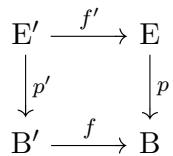
\includegraphics[keepaspectratio]{images/part002_b7191fdb.jpg}}

be a cartesian square. Suppose that E is a covering of B and that the space B' is connected and locally path-connected. Let b' be a point of B' and \(b = f(b')\) . For \((\mathrm{E}', p')\) to be a trivializable covering of B', it is necessary and sufficient that, for every point x of the fibre \(E_b\), the image of \(\pi_1(p, x)\) contain the image of \(\pi_1(f, b)\) .

This follows from prop. 1 and I, p. 81, cor. 5 of prop. 6.

